\documentclass{beamer} 
\usetheme{metropolis}
% \usecolortheme{spruce}
\setlength{\parindent}{0cm}
\usepackage{color}
\usepackage[utf8]{inputenc}
\usepackage[spanish]{babel}
\usepackage{amsmath}
\usepackage{amsfonts}
\usepackage{amssymb}
\usepackage{graphicx}
\usepackage{ragged2e}
\usepackage{caption}
\usepackage{subcaption}
\usepackage{tikz}
\usepackage{tcolorbox}
\usepackage{float}

\newtcolorbox{informacion}[2][]
{
  breakable,
  colframe = blue!5!white,
  colback  = blue!5!white,
  coltitle = blue!80!black,
  title    = \faInfo \hspace{5 mm} #2,
}


\title{
{\Large Mecánica de Materiales} \\
{\large III. Flexión}
}
\author{Pedro Jorge De Los Santos}
\institute{
    {\bf 
    Instituto Tecnológico de Celaya \\
    Departamento de Ingeniería Mecánica \\
    }
}

\apptocmd{\frame}{}{\justifying}{}
\begin{document}

\begin{frame}
\titlepage
\end{frame}

% Sección introducción
\section{Flexión}

\begin{frame}
\justifying
\frametitle{Introducción}

En ingeniería se denomina flexión al tipo de deformación que presenta un elemento estructural alargado en una 
dirección perpendicular a su eje longitudinal. El término \textit{alargado} se aplica cuando una dimensión es dominante 
frente a las otras. Un caso típico son las vigas, las que están diseñadas para trabajar, principalmente, por flexión.

\begin{center}
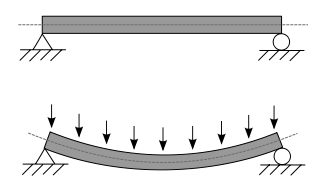
\includegraphics[width=0.6\textwidth]{img/bending.png}
\end{center}
\end{frame}


\begin{frame}
\justifying
\frametitle{Tipos de flexión}

\textbf{Flexión pura.} Flexión de la viga ante un momento flexionante

\begin{center}
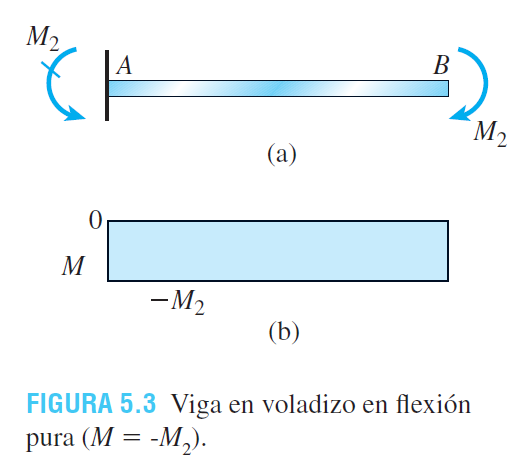
\includegraphics[width=0.55\textwidth]{img/viga_flexion_pura.PNG}
\end{center}
\end{frame}



\begin{frame}
\justifying
\frametitle{Tipos de flexión}

\textbf{Flexión no uniforme}. Flexión en presencia de fuerzas cortantes

\begin{center}
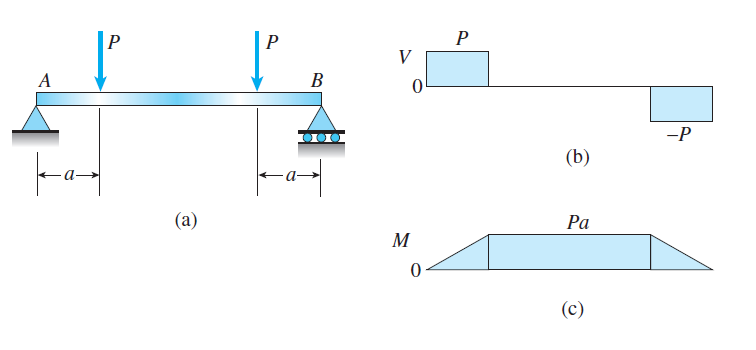
\includegraphics[width=0.9\textwidth]{img/viga_flexion_no_uniforme.PNG}
\end{center}
\end{frame}



\begin{frame}
\justifying
\frametitle{Flexión}

$$ P = P' $$
$$ M = Px $$

\begin{center}
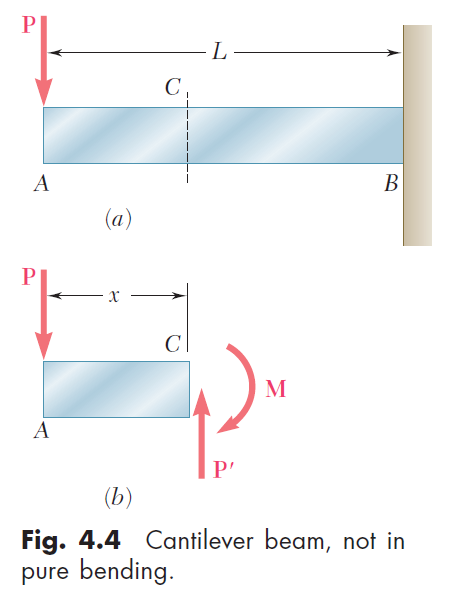
\includegraphics[width=0.37\textwidth]{img/cantiliver_beam.PNG}
\end{center}

\end{frame}


\begin{frame}
\justifying
\frametitle{Flexión}
La distribución de esfuerzos normales en la sección puede obtenerse del par $\mathbf{M}$ como 
si la viga estuviese en flexión pura.

\hfill \\

Los esfuerzos cortantes en la sección dependen de la fuerza  $P'$.

\end{frame}



\begin{frame}
\justifying
\frametitle{Elemento simétrico sometido a flexión pura}

Las fuerzas internas en cualquier sección transversal de un elemento simétrico 
en flexión pura son equivalentes a un par. El momento $M$ se conoce como 
\textit{momento flector}.

\begin{center}
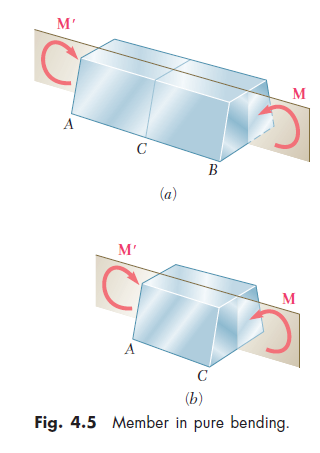
\includegraphics[width=0.4\textwidth]{img/member_pure_bending.PNG}
\end{center}

\end{frame}


\begin{frame}
\justifying
\frametitle{Signo del momento flector}

Dependiento la curvatura que produzca.

\begin{center}
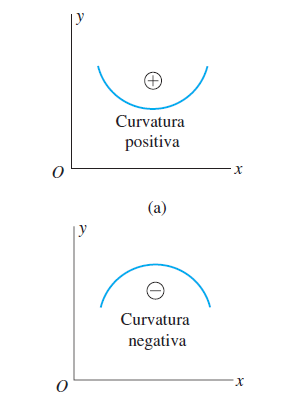
\includegraphics[width=0.4\textwidth]{img/signo_curvatura.PNG}
\end{center}
\end{frame}



\begin{frame}
\justifying
\frametitle{Deformaciones en un elemento simétrico sometido a flexión pura}

En cualquier punto de un elemento delgado, en flexión pura, se tiene un estado de esfuerzo 
uniaxial. Dado AB decrece y A'B' se alarga, cuando $M>0$, se nota que la deformación $\epsilon_x$ y 
el esfuerzo $\sigma_x$ son negativos en la parte superior del elemento (compresión) y positivos en la 
parte inferior (tensión).

\begin{center}
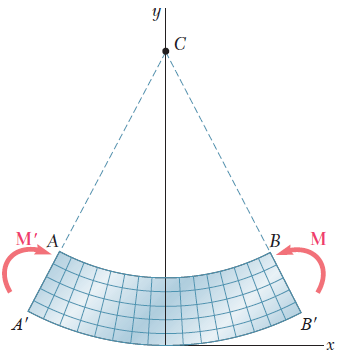
\includegraphics[width=0.4\textwidth]{img/longitudinal_section.PNG}
\end{center}
\end{frame}



\begin{frame}
\justifying
\frametitle{Deformaciones en un elemento simétrico sometido a flexión pura}

Existe una superficie paralela a las caras superior e inferior del elemento, donde 
$\epsilon_x$ y $\sigma_x$ se anulan, conocida como superficie neutra.

\begin{center}
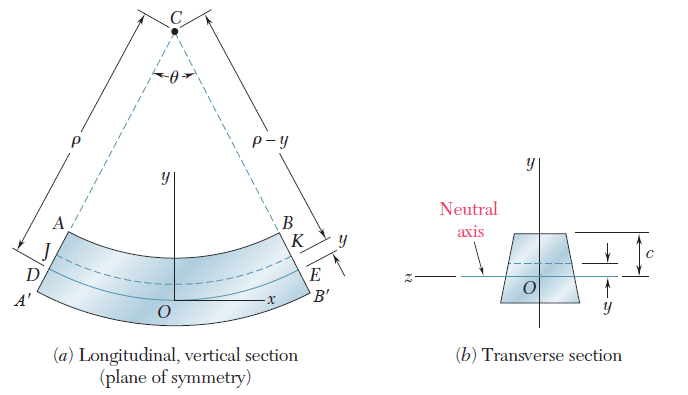
\includegraphics[width=0.8\textwidth]{img/deformation_neutral_axis.PNG}
\end{center}
\end{frame}



\begin{frame}
\justifying
\frametitle{Deformaciones en un elemento simétrico sometido a flexión pura}

Considerando el eje neutro:

$$ 
L = \rho \theta
$$

Considerando el arco JK:

$$ L' = (\rho - y) \theta $$

Dado que inicialmente la longitud de JK era igual a L, entonces:

$$ \delta = L' - L $$
\end{frame}



\begin{frame}
\justifying
\frametitle{Deformaciones en un elemento simétrico sometido a flexión pura}

Sustituyendo:

$$  \delta = (\rho - y) \theta - \rho\theta $$

La deformación unitaria longitudinal $\epsilon_x$ de los elementos de JK 
se obtiene dividiendo $\delta$ entre la longitud original $L$ de JK:

$$ \epsilon_x = \frac{\delta}{L} = \frac{-y\theta}{\rho\theta} $$

$$ \epsilon_x= - \frac{y}{\rho} $$
\end{frame}



\begin{frame}
\justifying
\frametitle{Deformaciones en un elemento simétrico sometido a flexión pura}

Si $c$ es la distancia máxima a la superficie neutra, y $\epsilon_m$ el valor máximo absoluto de 
la deformación unitaria, entonces:

$$ \epsilon_m = \frac{c}{\rho} $$

Luego:

$$ \epsilon_x = -\frac{y}{c}\epsilon_m $$
\end{frame}



\begin{frame}
\justifying
\frametitle{Esfuerzos y deformaciones en el rango elástico}

Si $c$ es la distancia máxima a la superficie neutra, y $\epsilon_m$ el valor máximo absoluto de 
la deformación unitaria, entonces:

$$ \epsilon_m = \frac{c}{\rho} $$

Luego:

$$ \epsilon_x = -\frac{y}{c}\epsilon_m $$
\end{frame}



\begin{frame}
\frametitle{Referencias}

\begin{enumerate}
\item Beer, F. P. (2013). Mecánica de materiales. México, D.F: McGraw-Hill Interamericana.
\item Gere, J. M., Goodno, B. J., & León, C. J. (2014). Mecánica de materiales. Australia: Thomson Learning.
\item Gere, J., & Timoshenko, S. (1998). Mecǹica de materiales. Mx̌ico, D.F: Thomson Learning.
\item Hibbeler, R. C., Murrieta, M. J. E., Molina, S. O., & Saldaña, S. S. (2011). Mecánica de materiales. Naucalpan de Juárez, México: Pearson educación.
\end{enumerate}
\end{frame}

\begin{frame}
\justifying
\frametitle{...}

El contenido de esta presentación está basado en las referencias bibliográficas básicas del curso. 
Si no se indica de manera explícita, las imágenes y diagramas corresponden a la referencia [1].

\end{frame}


\end{document}

